\chapter{Configuring your MEGA65}
\label{cha:configuring}

\section{Preparing for First Use: Formatting SD Cards}

Depending on the model, your MEGA65 may or may not come with a pre-configured SD card.
If it doesn't, or if you wish to use a different SD card, e.g., with a
larger capacity, you must first format it for use in the MEGA65.

{\em This must be done in the MEGA65, not in a PC or other computer!}

There are several reasons for this: First, in order to fit the most
features into the MEGA65's small operating system, it is a little bit
particular about the FAT32 file system it uses. Second, only the
MEGA65 FDISK/FORMAT utility can create a MEGA65 System Partition. The
MEGA65 System Partition holds non-volative configuration settings for
your MEGA65, and also contains the freeze slots, that make it easy to
switch which programme or game you are running on your MEGA65.

Fortunately, formatting an SD card on the MEGA65 is very easy.

First, power the MEGA65 on while holding the \megakey{ALT} key down.
This should present you with the MEGA65 Utility Menu, which contains a
selection of built-in utilities, similar to the following:

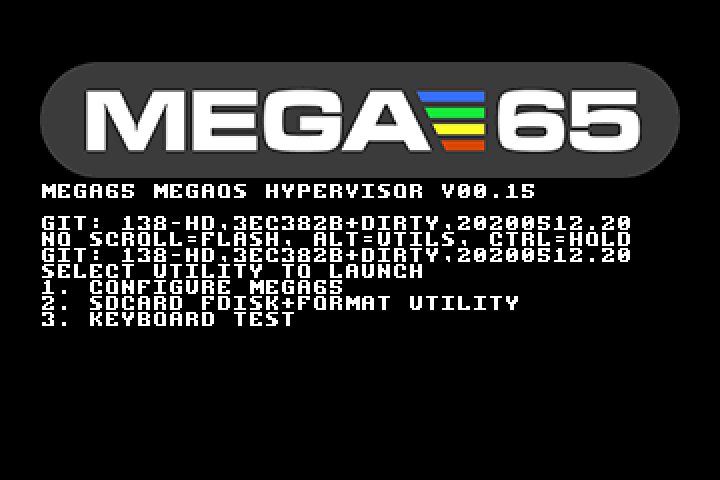
\includegraphics[width=\linewidth]{images/ss-utilmenu.png}

The exact set of utilities will
depend on the model of your MEGA65 and the version of the MEGA65
factory core which it is running. However, all versions include both
the MEGA65 FDISK/FORMAT utility, and the MEGA65 Configure utility.
Most models also include a keyboard test utility, that you can use at
any time to test that your keyboard is functioning correctly.  This is
in fact the same utility that used in the factory when testing brand
new keyboards.

Select the number that corresponds to the FDISK/FORMAT utility.  This
will typically be 1.  The FDISK utility will start, and attempt to
detect the size of any SD cards you have installed.  If you have both
an internal and external SD card installed, it will allow you to
choose which one you wish to format. The internal SD card is bus 1,
and the external card is bus 0.  But note that the MEGA65 will
always attempt to boot using an external microSD card, if one is
installed.

For safety when formatting we {\em strongly} recommend
that you remove any SD card or microSD card that you do not intend to
format, so that you can't accidently destroy any data.  This is
because formatting an SD card in the MEGA65 cannot be undone, and you
{\em WILL} lose all data that is currently on the SD card.  If you
have any files or data on the SD card that you wish to retain, you
should first back this up somewhere.  The contents of the FAT32
partition can be easily backed up by inserting the SD card into
another computer.  The contents of the MEGA65 System Partition,
including the contents of freeze slots requires the use of specialised
software.

In generaly, you should aim to backup any valuable data from your
MEGA65 on a regular basis, especially while the computer remains under
development.  While we take every care to avoid data corruption or
other mishaps, we can't guarantee that the MEGA65 is free of bugs in
this regard.

If you have only an internal SD card, you might see a
display similar to the following:

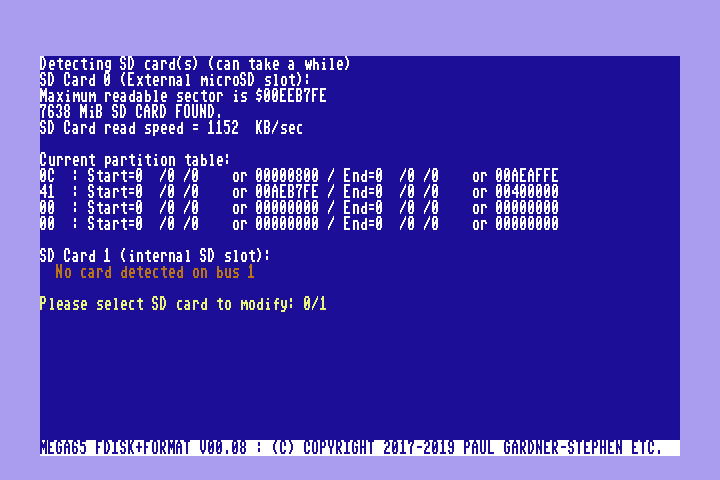
\includegraphics[width=\linewidth]{images/ss-m65fdisk-busselect.png}

Once you have selected the bus, the FDISK/FORMAT utility will ask you
to confirm that you wish to delete everything:

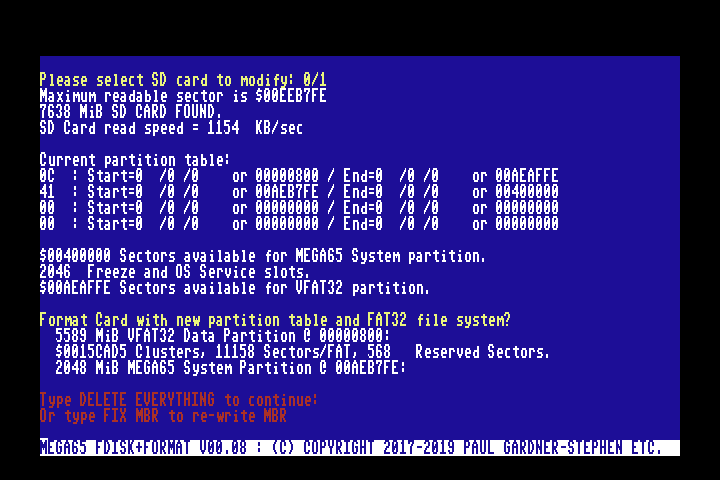
\includegraphics[width=\linewidth]{images/ss-m65fdisk-typesomething.png}

To make sure that you
know what you are doing, and don't accidentally delete everything, you
must type in ``DELETE EVERYTHING'' in capitals and press
\megakey{RETURN}.  Alternative, you can turn the MEGA65 off and on to
abort this process, without causing any damage to your data.

It is also possible to attempt to recover from a lost Master Boot
Record (``Boot Sector'') by instead typing ``FIX MBR,'' should the
need arise.

\section{Installing ROM and Other Support Files}

The MEGA65 FDISK/FORMAT utility will install a version of the
open-source OpenROM project's C64-compatible ROMs as part of the
formatting process. However, you may have other ROMs that you wish to
use on the MEGA65. The 911001 version of the C65 ROM in
particular is known to work well with the MEGA65.
You can copy as many of these as you wish onto the
SD card.  Simply make sure that they have the .ROM extension.  The ROM
you wish to use by default should be called MEGA65.ROM.  These files
should be 128KB in size, and use the same internal format as ROMs
intended for the C65.  This means that the C64-mode KERNAL should be
placed at offset \$E000, a C65-mode BASIC at \$A000, and a suitable
character set at \$D000.  

Other important files include FREEZER.M65 and AUDIOMIX.M65, which
allow you to use the MEGA65's integrated freezer.  You can download
the full set of support files for the MEGA65 from:

\url{https://github.com/mega65/mega65-files}

